\section{Experiments}
VAEPP is evaluated in vast common datasets including MNIST, Fashion-MNIST~\cite{xiao2017/online}, CIFAR-10~\cite{krizhevsky2009learning} and CelebA with metrics log-likelihood, FID~\cite{heusel2017gans} and IS~\cite{salimans2016improved} to show the performance of VAEPP. Moreover, we try to help VAE to solve OoD problem by the additional information of discriminator. 
\subsection{Log-likelihood}
\begin{table}[tb]
\centering
\begin{tabular}{lrr}  
\toprule
Model  &  MNIST & CIFAR\\
\midrule
\textbf{With autoregressive}   \\
PixelCNN         &  81.30  &  3.14   \\
DRAW             &  80.97  &  3.58    \\
IAFVAE           &  79.88  &  3.11    \\
PixelVAE++       &  78.00  &  2.90   \\
PixelRNN         &  79.20  &  3.00    \\
VLAE             &  79.03  &  2.95     \\
PixelHVAE with VampPrior &  78.45  &     \\
\midrule
\textbf{Without autoregressive}   \\
Discrete VAE     &  81.01     \\
LARS             &  80.30     \\
VampPrior        &  79.75     \\
Naive VAEPP      &  79.18 & 3.15    \\
VAEPP            &  77.46 & 2.91	    \\
VAEPP+Flow       &  77.11 & 2.84    \\
\bottomrule
\end{tabular}
\caption{Test log-likelihood on MNIST and Bits/dim on CIFAR-10. Bits/dim means $-\log p_\theta(x|z) / (3072 * \ln(2))$. Most of VAEs based on learnable prior focus on MNIST and don't try CIFAR-10. 
%The learnable prior is indeed more useful on MNIST since the reconstruction loss is not hard to optimize on MNIST and the improvement by autoregressive component is limited. On CIFAR-10, the image is more complex and reconstruction loss is hard to optimize. Therefore, autoregressive component improve the VAEPP significantly and the improvement of learnable prior is limited. 
VAEPP+Flow means that we apply a normalization flow on encoder, to enhance the ability of encoder. 
Additional, we compare VAE based on $q_\phi(z|x)$ and $q_\phi(z|e)$ on MNIST, whose NLL are 81.10 and 83.30 respectively. It validates that using $q_\phi(z|e)$ is not the reason of improvement but the powerful presentation ability of Pull-back Prior. VAEPP achieves the state of art on MNIST, and is competitive to the models with autoregressive component. }
\label{tab:mnist-nll}
\end{table}
\begin{table}[tb]
\centering
\begin{tabular}{lrrr}  
\toprule
Model   & Static MNIST & Fashion & Omniglot \\
\midrule
Naive VAEPP    &  81.16    &  225.08  &  96.86  \\
VAEPP          &  79.85    &  222.42  &  88.85   \\
VAEPP+Flow     &  80.77    &  222.23  &  88.83   \\
\bottomrule
\end{tabular}
%Naive VAEPP    &  81.16$\pm$    &  225.08$\pm$1.18  &  96.86$\pm$  \\
%VAEPP          &  79.85$\pm$    &  222.42$\pm$1.57  &  88.85$\pm$   \\
%VAEPP+Flow     &  80.77$\pm$    &  222.23$\pm$1.39  &  88.83$\pm$   \\
\caption{Test log-likelihood on Static MNIST, Fashion-MNIST and Omniglot. VAEPP+Flow get better loss in Static MNIST than VAEPP but it suffers from overfitting, which leads to worse test log-likelihood. }
\label{tab:cifar-nll}
\end{table}
We evaluate and compare the performance of VAEPP after training by \cref{alg:vaepp} and \cref{alg:improved_vaepp} on CIFAR10 when the garadient penalty algorithm is selected from 3 strategy: WGAN-GP, WGAN-div-1  (sampling the linear combination of two real or two fake data points), WGAN-div-2 (sampling both real or fake data points) as shown in \cref{tab:compare_nD_over_R}. Our conclusion is that \cref{alg:improved_vaepp} outperforms \cref{alg:vaepp} under all of settings in CIFAR-10 dataset. We then evaluate them on other datasets, MNIST, CelebA. This conclusion also holds for them. This validate our proposition in \cref{subsec:improve_of_vaepp}. 
\begin{table}[tb]
\centering
\begin{tabular}{lrr}  
\toprule
GP Strategy  &  Naive VAEPP  & VAEPP \\
\midrule
WGAN-GP      &  3.15   & 2.95      \\
WGAN-div-1   &  3.20   & 2.91      \\
WGAN-div-2   &  4.47   & 2.99      \\
\bottomrule
\end{tabular}
\caption{Comparation between VAEPP and Improved VAEPP when gradient penalty strategy varies on CIFAR-10 with dim $\mathcal{Z} = 1024$. For any gradient penalty strategy in the table, VAEPP outperforms Naive VAEPP, which validates the our intuition of design of \cref{alg:improved_vaepp}. We select WGAN-div-1 as our default gradient penalty strategy since it achieves best performance in VAEPP. Although WGAN-GP outperforms WGAN-div-1 in Naive VAEPP, the difference is acceptable (3.20 and 3.15 is both not good enough) and Naive VAEPP is not the final algorithm. }
\label{tab:compare_nD_over_R}
\end{table}

We compare our algorithms with other log-likelihood based model on MNIST, CIFAR-10 and CelebA as shown in \cref{tab:mnist-nll}, \cref{tab:cifar-nll}. Because the improvement of auto-regressive components is significant, we separate models by whether use auto-regressive component as \cite{maaloe2019biva} did. Improved VAEPP outperforms most of the models without autoregressive component and is competitive to the models with autoregressive component. The reason of why VAEPP don't use auto-regressive component is that VAEPP is time-consuming in training,  evaluation and sampling due to the huge structure (need additional discriminator) and Langevin dynamics. It is not easy to apply auto-regressive component on VAEPP considering auto-regressive component is also time-consuming. 
% Concretely, a whole process including training, evaluation and sampling on CIFAR10 will cost roughly one week on single Nvidia 2080Ti GPU card. 
On the other hand, we expect that the pure improvement on learnable prior could improve the performance of VAE rather than the careful design on encoder or decoder, since it is clearer and easier to develop in theory. Therefore, how to apply autoregressive component on VAEPP is a valuable and challenging practical work. We leave it as a future work.

To valid that it is better to use $q_\phi(z)$ to evaluate $Z$ than $p_\mathcal{N}(z)$ in ~\cref{subsec:determine_z}, we calculate the $KL(q_\phi(z)||p_\lambda(z))$ and $KL(p_\mathcal{N}(z)||p_\lambda(z))$ on CIFAR-10 and MNIST. The former is less than the difference (180.3 on CIFAR-10) between reconstruction loss and ELBO and the latter one can be evaluated directly (1011.30 on CIFAR-10). Consequently, $q_\phi(z)$ is closer to $p_\lambda(z)$ than $p_\mathcal{N}(z)$. 

To valid that VAEPP is more stable and efficient than Naive VAEPP in \cref{subsec:improve_of_vaepp}, we draw the training loss of VAEPP and Naive VAEPP on CIFAR-10, shown in fig (TODO).
%We evaluate $Z$ by two ways mentioned in \cref{subsec:determine_z} and compare the variance of them in 10 times on CIFAR-10. The variance of estimation based on $q_\phi(z)$ (4.82), is much less than the variance of estimation based on $p_\mathcal{N}$ (TODO), which supports our proposition in \cref{subsec:determine_z}. Since the variance of $Z$ also influence the variance of log-likelihood, we also evaluate the variance of log-likelihood in 10 times on CIFAR-10 (4.82) to ensure the stability of evaluation. 

\subsection{Quality of Sampling}
The quality of samples of VAE is worse than GAN, and it is indeed a reason that we involve the techniques of GAN to improve the VAE model. We apply Wasserstein distance to infer Pull-back Prior and GAN to sample the initial $z_0$ for Langevin dynamics. These techniques will help VAEPP improve the quality of samples. The samples of VAEPP gets good FID and IS, competitive to GANs and 2-Stage VAE (which is the SOTA of VAE in FID). 
\begin{table}[tb]
\centering
\begin{tabular}{lrrrrrrr}  
\toprule
Model & MNIST & Fashion & CIFAR & CelebA\\
\midrule
Best GAN   & $\sim10$& $\sim32$&$\sim70$& $\sim49$\\
VAE+Flow   & $54.8$. & $62.1$  & $81.2$ & $65.7$\\
WAE-MMD    & $115.0$ & $101.7$ & $80.9$ & $62.9$\\
2-StageVAE & $12.6$  & $29.3$  & $72.9$ & $44.4$\\
VAEPP      & $12.6$  & $29.3$  & $71.3$ & $55.0$ \\
\bottomrule
\end{tabular}
\caption{FID comparasons to GAN-based models and other VAEs. Best GAN indicates the best FID on each dataset across all GAN models when trained using settings suggested by original authors. The data of Best GAN and other VAEs is from \protect\cite{dai2019diagnosing}. As suggested by \protect\cite{dai2019diagnosing}, the variance of $p_\theta(x|z)$ of VAEPP is independent on $z$ and the dimension of latent space is small (128). }
\label{tab:compare_FID}
\end{table}
\begin{figure}
	\centering
	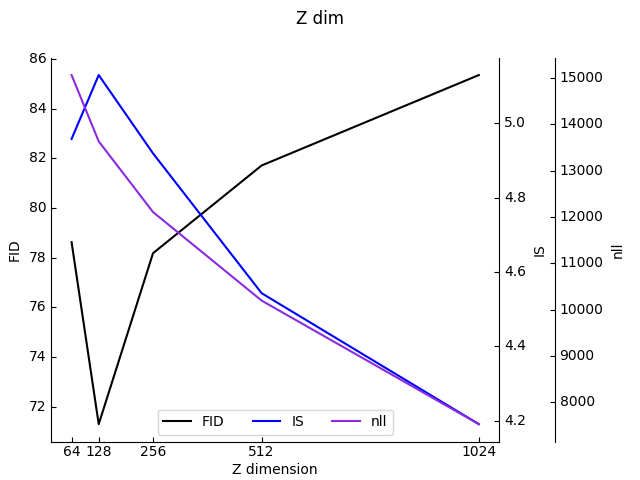
\includegraphics[width=0.5\columnwidth]{../figures/fid_is_nll_on_different_dim.png}
	\caption{
	Comparation of VAEPP when the dimension of latent space varies on CIFAR-10 with metrics log-likelihood, FID and IS.
	}
	\label{fig:compare_nD_over_z_dim}
\end{figure}

However, as common sense, it is hard to achieve best performance in FID, IS and log-likelihood by same setting. We observe this fact that when dimension of latent space is increasing, the FID, IS become worse, as shown in \cref{fig:compare_nD_over_z_dim}. The trend of FID, IS is different to the trend of log-likelihood, which is increasing when dimension of latent space is increasing, as shown in \cref{fig:compare_nD_over_z_dim}. As diagnosis in \cite{dai2019diagnosing}, the dimension of latent space should be selected as a number that little larger than the dimension of real data manifold, suggested by their experiment, dim $\mathcal{Z}$ = 64, same as our experimental result.  

To valid the \cref{eq:behavior_of_beta}, we calculate the $\E_{p_\lambda(z)}[ D(G(z))]$ (discriminator on generated samples) and $\E_{q_\phi(z)}[ D(G(z))]$ (discriminator on reconstructed samples). They are -12.3467 and -12.2947 respectively on CIFAR-10. The discriminator on real samples are -12.2962, which is near same as discriminator on reconstructed samples. 

% CIFAR [-12.352115, -12.347757, -12.345433, -12.345455, -12.3524475, 
% -12.345604, -12.345031, -12.348698, -12.346703, -12.350895, -12.353839,
% -12.3432255, -12.342315, -12.346496, -12.341743, -12.346189, -12.354458, 
% -12.340977, -12.341134, -12.343964, -12.348272, -12.349046, -12.338009,
% -12.350307, -12.359574, -12.354169, -12.354169, -12.341797, -12.34804,
% -12.349505, -12.348672, -12.350969, -12.34367, -12.34062, -12.347913,
% -12.340741, -12.340741, -12.343849, -12.337844, -12.339806, -12.347616,
% -12.347033, -12.347033, -12.347033, -12.34675, -12.346854, -12.349438,
% -12.351765, -12.348437, -12.3403635, ] 
% http://mlserver.ipwx.me:7897/5e0a3a1642d74cd7474dc164/



\subsection{Out-of-Distribution}

We found that discriminator of VAEPP performs normally while model assign higher density to the data from out-of-distribution, as shown in fig(TODO). It inspires us to use the exact information from discriminator to design 3 indicators, log-likelihood $\log p_\theta(x)$, energy $D(x)$ and norm of gradient $\|\nabla_{x} D(x)\|$ to solve OoD problem, as shown in fig(). From the likelihood, \cite{song2017pixeldefend} showed that it is useful to assume the data is out-of-distribution if it have very high or very low density. For energy and norm of gradient, it performs normally, i.e., when energy is higher or norm of gradient is smaller, it more likely belongs to out-of-distribution. Hence, we evaluate the AUC and AP for them and combination of them in OoD problem on CIFAR and SVHN, as shown in \cref{tab:compare_ood}. The method to combine them is simple: normalize them into a standard Gaussian in training set of CIFAR, and the score of this indicator contributing to combination score is the absolute/original/negative value of it. We have tested all kinds of combination and the best one is $|\log p_\theta(x)| - \|\nabla_x D(x)\|$. The performance of it on other datasets is shown in \cref{tab:compare_ood_other_datasets} which is competitive to other indicators $T_{perm}$~\cite{song2017pixeldefend} and WAIC~\cite{choi2018waic}. 
\begin{table}[tb]
\centering
\begin{tabular}{lrr}  
\toprule
Indicator  & AUC/AP \\
\midrule
$\log p_\theta(x)$   &  1.00/1.00      \\
$D(x)$               &  1.00/1.00      \\
$\|\nabla_x D(x)\|$  &  1.00/1.00      \\
$|\log p_\theta(x)| - \|\nabla_x D(x)\|$ & 1.00/1.00 \\
\bottomrule
\end{tabular}
\caption{Comparation between indicators and their combination.}
\label{tab:compare_ood}
\end{table}
\begin{table}[tb]
\centering
\begin{tabular}{lrrrr}  
\toprule
Dataset  &  $T_{perm}$ & WAIC & VAEPP\\
\midrule
Fashion vs MNIST  & 0.78/0.71  & 0.24/0.38 & 1.00/1.00  \\
CIFAR vs SVHN     & 0.86/0.82  & 0.16/0.55 & 1.00/1.00  \\
CIFAR vs ImageNet & 0.50/0.51  & 0.58/0.59 & 1.00/1.00  \\
CIFAR vs LSUN     & 0.58/0.56  & 0.60/0.28 & 1.00/1.00  \\
\bottomrule
\end{tabular}
\caption{Comparation the performance of VAEPP with other models in OoD problem. The data of $T_{perm}$ and WAIC is from \protect \cite{song2019unsupervised}. The reason that we can't compare VAEPP with \protect\cite{song2019unsupervised} is that it assumes a batch of OoD data can be obtained but we don't have this assumption. In fast, many online anomaly detection system must deal the online data on time when the number of OoD data in a batch is unknown. }
\label{tab:compare_ood_other_datasets}
\end{table}

